\documentclass{article}
\usepackage[utf8]{inputenc}
%\usepackage[T1]{fontenc}
\usepackage{amsthm}
\usepackage{amsmath}
\usepackage{amssymb}
\usepackage{mathtools}
\usepackage{graphicx}
\newtheorem*{definition*}{Definition}
\newtheorem*{property*}{Property}
\newcommand\sbullet[1][.5]{\mathbin{\vcenter{\hbox{\scalebox{#1}{$\bullet$}}}}}
\DeclarePairedDelimiter{\norm}{\lVert}{\rVert}
\DeclarePairedDelimiter{\abs}{|}{|}
\newcommand*{\vertbar}{\rule[-1ex]{0.5pt}{2.5ex}}
\newcommand*{\horzbar}{\rule[.5ex]{2.5ex}{0.5pt}}
\usepackage{pdfpages}

\usepackage{hyperref}
\hypersetup{
  colorlinks=true,
  linkcolor=blue,
  filecolor=magenta,      
  urlcolor=cyan,
}



\author{phunc20}
\title{Recurrent neurons (p.381)}
%\date{January 21, 2021}

\begin{document}

\maketitle
%\tableofcontents

\begin{abstract}
Personally, I found the equations on p.381 were not to the point, at least not enough for me to grasp the exact
meaning and shapes of the input and output of a layer of recurrent neurons. Every time I re-read these paragraphs,
I cannot recall the understanding I reached at the previous reading. Thus, I decided to make a note here to try
to change the situation, hoping to make things clearer.
\end{abstract}

\section{A Single Recurrent Neuron}
The output of a single recurrent neuron of a single input instance $x_{(t)}$ equals
$$
  y_{(t)} = \phi\bigg(
    \langle x_{(t)}, w_x \rangle
    + y_{(t-1)} w_y
    + b
  \bigg)\,,
$$
where
\begin{itemize}
  %\item $x_{(t)}, w_x \in \mathbb{R}^{n_{\text{input}}}$ ($n_{\text{input}}$ can be any positive integer the user consider suitable)
  \item $x_{(t)}, w_x \in \mathbb{R}^{k}$ ($k$ can be any positive integer the user consider suitable)
  \item $\langle \cdot\,, \cdot \rangle$ denotes the inner product in $\mathbb{R}^k$
  \item $y_{(t-1)} \in \mathbb{R}$ is the output of the previous time step
  \item $w_y, b$ are both in $\mathbb{R}$
\end{itemize}




\newpage
%\thispagestyle{empty}


%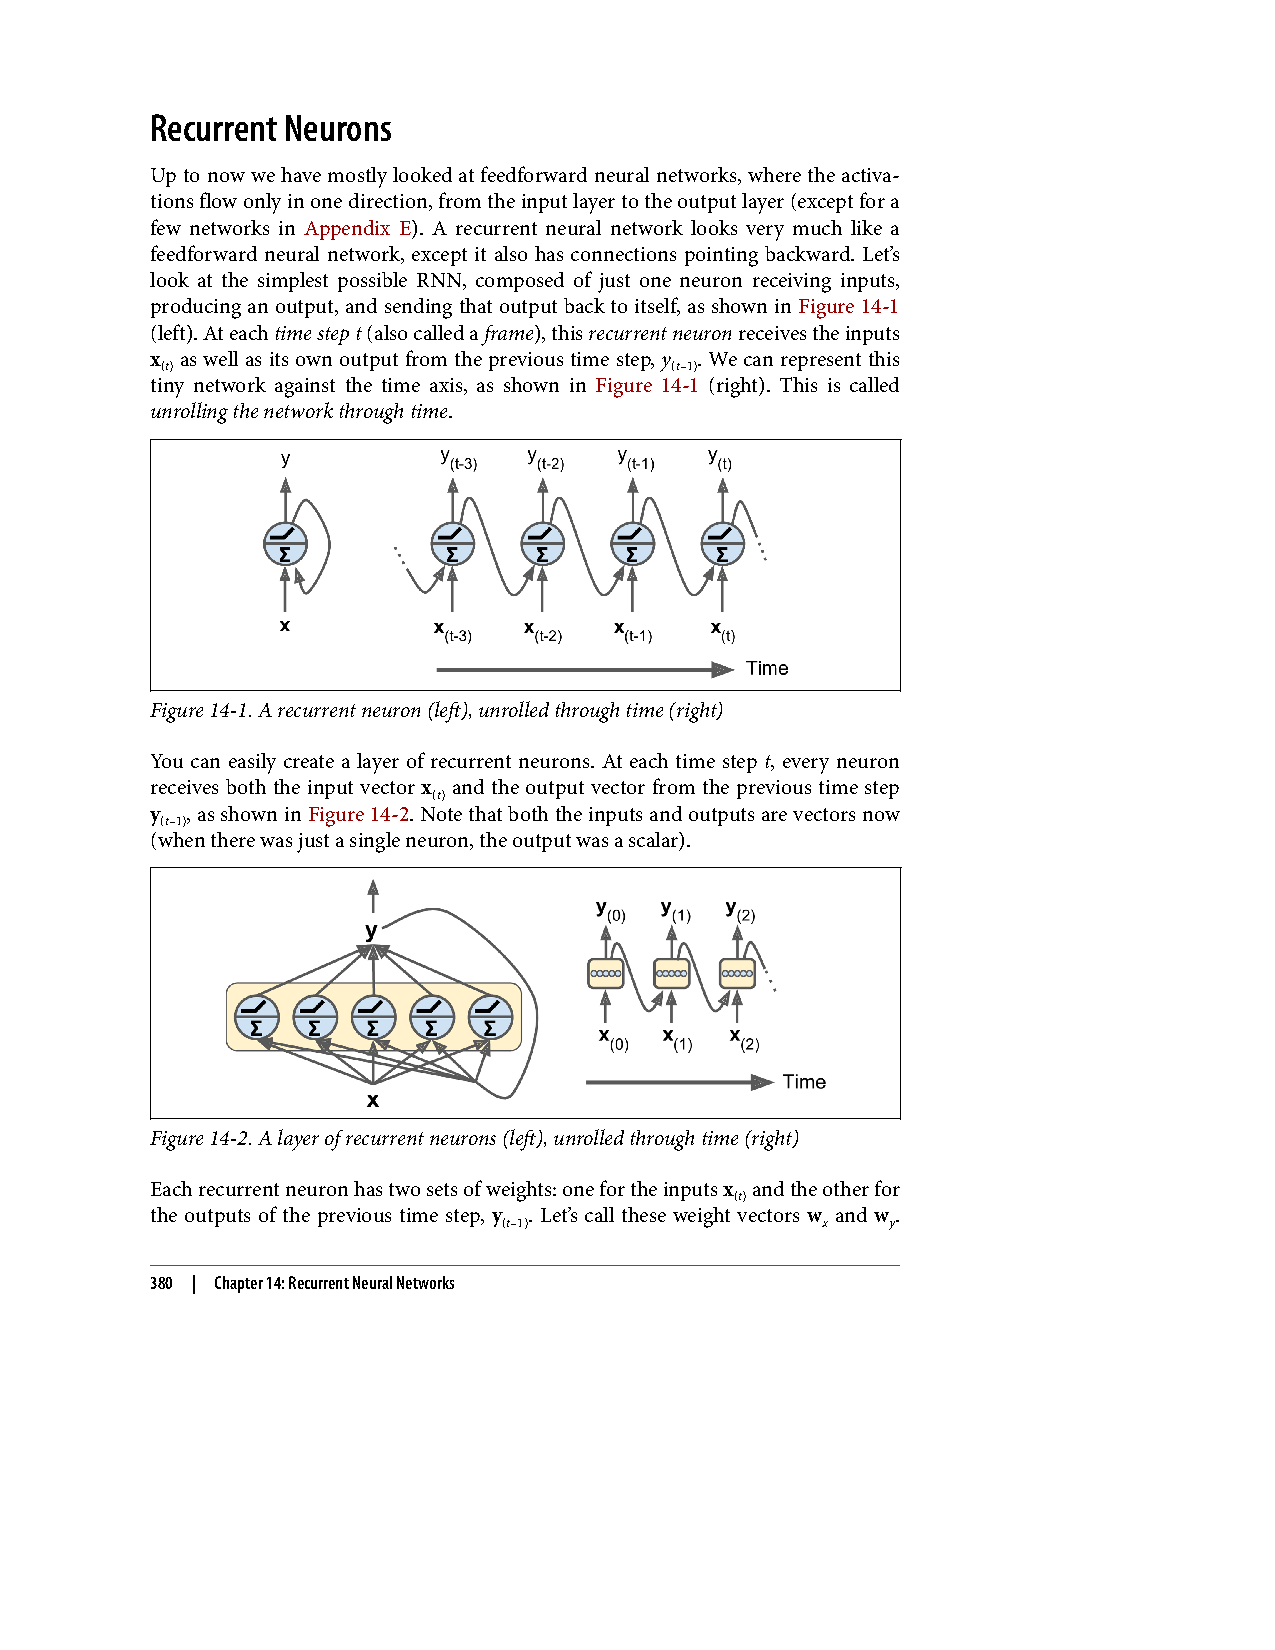
\includepdf[pages={1}]{p380.pdf}
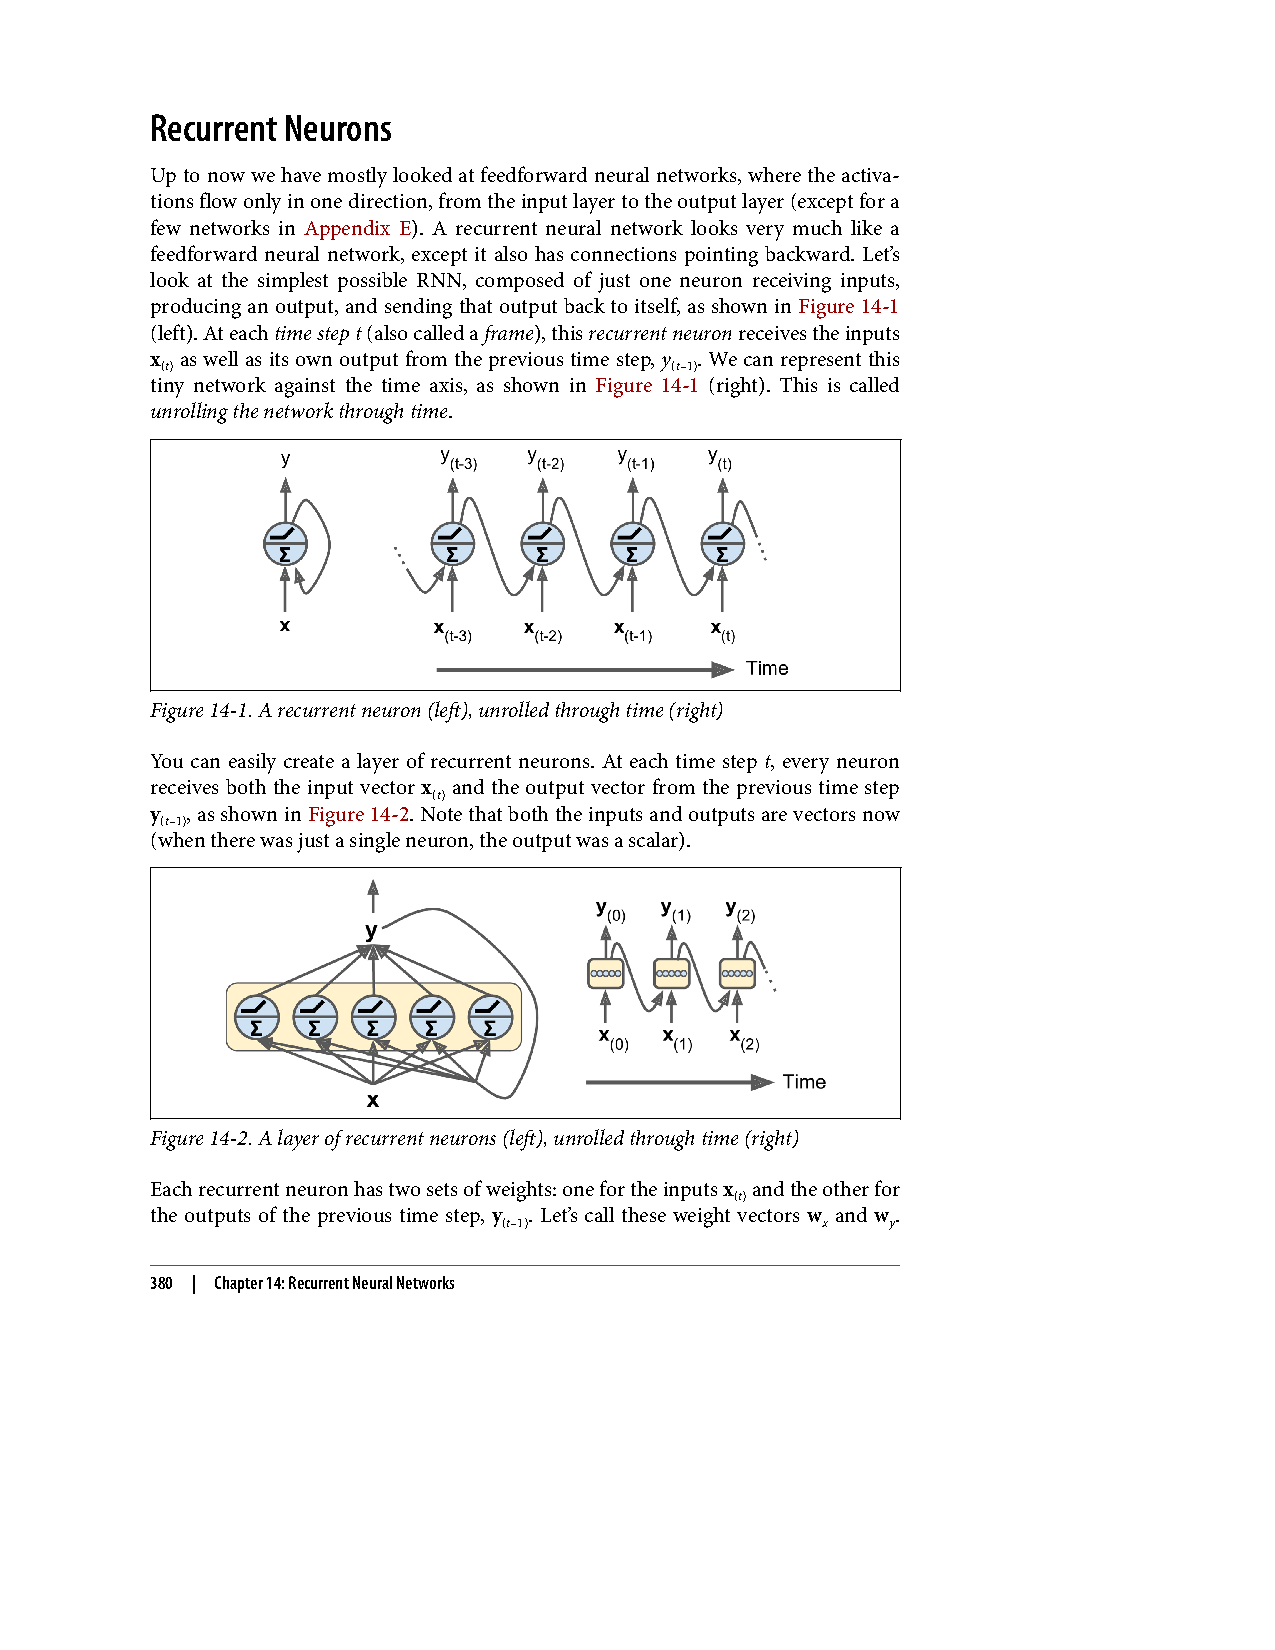
\includepdf[pages=-]{p380-381.pdf}


\setcounter{page}{4}

\section{A Layer of Recurrent Neurons}
To illustrate, let's take Figure 14-2 for example, in which we have a layer of \textbf{5} recurrent neurons. So,
the output of this particular layer equals
\begin{align*}
  \begin{pmatrix}
    y_{(t), 1} \\
    y_{(t), 2} \\
    y_{(t), 3} \\
    y_{(t), 4} \\
    y_{(t), 5}
  \end{pmatrix}
  &= \phi
  %\Bigg(\begin{bmatrix}
  \begin{pmatrix}
    \langle x_{(t)}, w_{x, 1} \rangle
    + \langle y_{(t-1)}, w_{y, 1} \rangle
    + b_1 \\
    \langle x_{(t)}, w_{x, 2} \rangle
    + \langle y_{(t-1)}, w_{y, 2} \rangle
    + b_2 \\
    \langle x_{(t)}, w_{x, 3} \rangle
    + \langle y_{(t-1)}, w_{y, 3} \rangle
    + b_3 \\
    \langle x_{(t)}, w_{x, 4} \rangle
    + \langle y_{(t-1)}, w_{y, 4} \rangle
    + b_4 \\
    \langle x_{(t)}, w_{x, 5} \rangle
    + \langle y_{(t-1)}, w_{y, 5} \rangle
    + b_5 \\
  \end{pmatrix}, \;\text{i.e.} \\
  %\end{bmatrix}\Bigg), \;\text{i.e.} \\
  y_{(t)} &= \phi\bigg(
    {W_{x}}^{T}\, x_{(t)} + {W_{y}}^{T}\, y_{(t-1)} + b
  \bigg),
\end{align*}
where
\begin{itemize}
  \item $y_{(t), j} \in \mathbb{R}$ for all $j=1,2,3,4,5$
  %\item $x_{(t)} \in \mathbb{R}^{k}$ as before, and $y_{(t-1)} \in \mathbb{R}^{l},$ where $l =$ \#(recurrent neurons).
  \item $x_{(t)} \in \mathbb{R}^{k}$ as before, and $y_{(t-1)} \in \mathbb{R}^{l},$ where $l = \text{\#(recurrent neurons)}$, i.e. number of recurrent neurons in the layer, here, in particular, $l=5$
  \item $w_{x,j} \in \mathbb{R}^k, w_{y,j} \in \mathbb{R}^l, b_{j} \in \mathbb{R}$ are the weights and bias associated with the $j$-th neuron (for all $j=1,2,3,4,5$)
  \item We define
    \begin{align*}
      {W_x}^{T} &= \begin{pmatrix}
        \quad\horzbar\;{w_{x,1}}^T{}\;\horzbar\quad \\
        \quad\horzbar\;{w_{x,2}}^T{}\;\horzbar\quad \\
        \quad\horzbar\;{w_{x,3}}^T{}\;\horzbar\quad \\
        \quad\horzbar\;{w_{x,4}}^T{}\;\horzbar\quad \\
        \quad\horzbar\;{w_{x,5}}^T{}\;\horzbar\quad \\
      \end{pmatrix} \\
      \\
      \qquad &{}\text{or equivalently} \\
      \\
      {W_x} &= \begin{pmatrix}
        \vertbar & \vertbar & \vertbar & \vertbar & \vertbar \\
        w_{x,1} & w_{x,2} & w_{x,3} & w_{x,4} & w_{x,5} \\
        \vertbar & \vertbar & \vertbar & \vertbar & \vertbar
      \end{pmatrix}\,.
    \end{align*}
  \item We define similarly
    \begin{align*}
      {W_y}^{T} &= \begin{pmatrix}
        \quad\horzbar\;{w_{y,1}}^T{}\;\horzbar\quad \\
        \quad\horzbar\;{w_{y,2}}^T{}\;\horzbar\quad \\
        \quad\horzbar\;{w_{y,3}}^T{}\;\horzbar\quad \\
        \quad\horzbar\;{w_{y,4}}^T{}\;\horzbar\quad \\
        \quad\horzbar\;{w_{y,5}}^T{}\;\horzbar\quad \\
      \end{pmatrix} \\
      \\
      \qquad &{}\text{or equivalently} \\
      \\
      {W_y} &= \begin{pmatrix}
        \vertbar & \vertbar & \vertbar & \vertbar & \vertbar \\
        w_{y,1} & w_{y,2} & w_{y,3} & w_{y,4} & w_{y,5} \\
        \vertbar & \vertbar & \vertbar & \vertbar & \vertbar
      \end{pmatrix}\,.
    \end{align*}
  \item It is understood that
    $$
    b =
    \begin{pmatrix}
      b_1 \\
      b_2 \\
      b_3 \\
      b_4 \\
      b_5
    \end{pmatrix}
    $$
\end{itemize}


\section{A Layer of Recurrent Neurons on A Batch of Instances}
Like in the case of a fully connected neural network, we can have an expression (using matrices) for
an entire batch of input instances, say, $m$ instances
\begin{align*}
  Y_{(t)} &= \phi\bigg(
    X_{(t)} W_x
    + Y_{(t-1)} W_y
    + b
  \bigg)
\end{align*}
where
\begin{itemize}
  \item $\texttt{shape(} X_{(t)}\texttt{)}= (m, k)$
  \item $\texttt{shape(} W_{x}\texttt{)}= (k, l)$
  \item $\texttt{shape(} Y_{(t-1)}\texttt{)}= (m, l)$
  \item $\texttt{shape(} W_{y}\texttt{)}= (l, l)$
  \item $\texttt{shape(} b\texttt{)}= (1, l)$
\end{itemize}


\end{document}
